\documentclass[11pt]{article}

%%%%%%%%%%%%%%Include Packages%%%%%%%%%%%%%%%%%%%%%%%%%%
\usepackage{xcolor}
\usepackage{mathtools}
\usepackage[a4paper, total={6in, 8in}, margin=1.25in]{geometry}
\usepackage{amsmath}
\usepackage{amssymb}
\usepackage{paralist}
\usepackage{rsfso}
\usepackage{amsthm}
\usepackage{wasysym}
\usepackage[inline]{enumitem}
\usepackage{hyperref}
\usepackage{tocloft}
\usepackage{titlesec}
\usepackage{colortbl}
\usepackage{wrapfig}
\usepackage{pdfpages}
\usepackage[american]{circuitikz}
%%%%%%%%%%%%%%%%%%%%%%%%%%%%%%%%%%%%%%%%%%%%%%%%%%%%%%%%



\begin{document}
\Large \noindent \textbf{Physics 5C Final Exam Review Session}\\
\normalsize
Department of Physics and Astronomy, UCLA\\

\noindent TA: Jinyan Miao (jnmiu@ucla.edu)\\
Review session: Thursday 5:00 - 6:30 PM (PST) over Zoom \\
Zoom ID: 963 5916 9873 (passcode: hiJinyan)\\
Click for the \href{https://ucla.zoom.us/j/96359169873?pwd=05p7ssCPwTbl8KfxoBNCOuaIbt68jW.1}{\underline{Zoom link}} and \href{https://sites.google.com/umich.edu/jmiu/worksheets}{\underline{solutions to the worksheets}}.\\
\noindent\rule{8cm}{0.4pt}\\

\noindent\textbf{Problem 1}: Jinyan keeps forgetting to plug in his cellphone, so he is building a wireless charging pad. In a simplified model, the receiver inside his phone is a circular coil with $N=25$ turns, radius $r=3.0\,$cm, and total resistance $R=2.0\,\Omega$. The coil lies flat in the plane of the page, and a uniform magnetic field produced by the charging pad points out of the page everywhere inside the coil. During one short time interval, the field strength decreases steadily from $B_i=1\,$T to $B_f=0.20\,$T in $\Delta t=0.5\,$s. Nothing in the phone is moving: The changing magnetic field produces a transformer emf in the receiver coil.

\begin{center}
\includegraphics[scale=0.69]{charger.pdf}
\end{center}

\noindent\textbf{Part (a)} Find the magnitude of the induced emf and the induced current in the coil.\\

\noindent\textbf{Part (b)} Determine whether the induced current is running clockwise or counterclockwise in the coil. In a few words, explain how this is determined.\\

\newpage
\noindent\textbf{Problem 2}: Jinyan wants to photograph a sunrise at Lake Michigan without too much glare, so he tests two ideal polarizing sheets in front of his camera. He first shines an unpolarized electromagnetic wave with average intensity $I_0=100\,\text{W/m}^2$ through the sheets. The first polarizer has a vertical transmission axis, while the second polarizer has a transmission axis at an angle $\theta$ from the vertical. His light sensor measures an intensity $I_2=20\,\text{W/m}^2$ after the second polarizer. Take
\begin{align*}
c=3.0\cdot 10^8\,\text{m/s}\,,\qquad
\epsilon_0=8.85\cdot 10^{-12}\,\text{F/m}\,.
\end{align*}

\noindent\textbf{Part (a)} Find the acute angle $\theta$ between the two transmission axes of the polarizers.\\

\noindent\textbf{Part (b)} Find the amplitudes of the oscillating electric field and magnetic field in the wave after it has passed through the second polarizer.\\

\noindent\textbf{Part (c)} Find the average total energy density in the original incident wave before it reaches either polarizer.

\newpage
\noindent\textbf{Problem 3}: Jinyan is testing a photoelectric detector for a UV safety sensor, but he has forgotten what metal was used inside it. He shines ultraviolet light with wavelength $\lambda=248\,$nm on the metal and finds that the fastest emitted electrons are stopped by a stopping potential of $V_{\text{stop}}=2.50\,$V. Take
\begin{align*}
h=6.63\cdot 10^{-34}\,\text{J}\cdot\text{s}\,,\qquad
c=3.0\cdot 10^8\,\text{m/s}\,,\\
1\,\text{eV}=1.6\cdot 10^{-19}\,\text{J}\,,\qquad
m_e=9.11\cdot 10^{-31}\,\text{kg}\,.
\end{align*}

\noindent\textbf{Part (a)} Find the work function (binding energy) $\phi$ of the metal in both eV and J.\\

\noindent\textbf{Part (b)} Find the longest wavelength of light that can eject electrons from this metal. Would red light with wavelength $620\,$nm eject any electrons? Explain your answer.\\

\noindent\textbf{Part (c)} Using the result from part (a), find the de Broglie wavelength of the fastest emitted electrons.\\

\hfill\break
\hfill\break
\hfill\break
\hfill\break
\hfill\break
\hfill\break
\hfill\break
\hfill\break
\hfill\break
\hfill\break
\noindent\textbf{Problem 4}: One of us has finished the Physics 5-series classes at UCLA and is now doing an internship at a local hospital. She receives a radioactive Iodine-131 sample that initially contains $N_0=6.4\cdot 10^{15}$ nuclei. Iodine-131 has a half-life of $t_{1/2}=8.0$ days.\\

\noindent\textbf{Part (a)} How many Iodine-131 nuclei remain after $12.0\,$ days?\\

\noindent\textbf{Part (b)} Find the activity of the sample at that time in Becquerels, where $1\,$Bq means one decay event per second.\\

\newpage
\noindent\textbf{Problem 5}: Jinyan is designing a 2-dimensional racetrack for charged particles. The racetrack consists of three components:
\begin{enumerate}[topsep=3pt,itemsep=-1ex,partopsep=1ex,parsep=1ex]
\item[A.] Region A is an empty space into which charges are launched;
\item[B.] Region B has a uniform magnetic field, where charges can make a U-turn;
\item[C.] Region C has a uniform electric field, where charges sprint towards the finish line.
\end{enumerate}
Neglect gravity and all types of friction in this problem.
\begin{center}
\includegraphics[scale=0.6]{racetrack}
\end{center}

\noindent\textbf{Part (a)} If the charges launched into region A are all negative, find the direction of the magnetic field in region B such that the charges turn and go towards region C. Then find the direction of the electric field in region C such that it accelerates the charges directly towards the finish line.\\

\noindent\textbf{Part (b)} Does the magnetic field in region B change the speed of a charge? What type of trajectory does a charge follow while it passes through region B? Explain briefly.\\

\noindent\textbf{Part (c)} A $q_1=-1\,$C charge with mass $m_1=2\,$kg is launched into region A with initial speed $1\,$m/s to the left. If the magnitude of the magnetic field in region B is $5\,$T, find the radius of the semi-circular path that the charge follows in region B.\\

\noindent\textbf{Part (d)} After the charge $q_1$ makes its U-turn, it enters region C with speed $1\,$m/s. Find the minimal strength of the electric field such that the charge crosses the finish line with speed $10\,$m/s. Assume that it travels $10\,$m in region C.


\newpage
\section*{Problem 1}
The key idea in this wireless-charging model is that the receiver coil does not move or change shape, but the magnetic field changes, so Faraday's law produces a transformer emf.\\

\noindent\textbf{Part (a)} The area enclosed by one turn of the coil is
\begin{align*}
A&=\pi r^2=\pi(3.0\cdot 10^{-2}\,\text{m})^2=2.83\cdot 10^{-3}\,\text{m}^2\,.
\end{align*}
The magnetic field is perpendicular to the plane of the coil, so it is parallel to the area normal vector and $\cos(0)=1$. The magnetic flux through one turn is therefore
\begin{align*}
\Phi_B=BA\,.
\end{align*}
The initial and final fluxes through one turn are
\begin{align*}
\Phi_{B,i}
&=(1.0\,\text{T})(2.83\cdot 10^{-3}\,\text{m}^2)
=2.83\cdot 10^{-3}\,\text{Wb}\,,\\
\Phi_{B,f}
&=(0.20\,\text{T})(2.83\cdot 10^{-3}\,\text{m}^2)
=5.65\cdot 10^{-4}\,\text{Wb}\,.
\end{align*}
Thus the flux change through one turn is
\begin{align*}
\Delta\Phi_B=\Phi_{B,f}-\Phi_{B,i}=5.65\cdot 10^{-4}\,\text{Wb}-2.83\cdot 10^{-3}\,\text{Wb}=-2.26\cdot 10^{-3}\,\text{Wb}\,.
\end{align*}
For a coil with $N$ turns, Faraday's law gives the magnitude of the induced emf,
\begin{align*}
\varepsilon=N\left|\frac{\Delta\Phi_B}{\Delta t}\right|=25\left|\frac{-2.26\cdot 10^{-3}\,\text{Wb}}{0.5\,\text{s}}\right|=0.113\,\text{V}\,.
\end{align*}
Using Ohm's law, the induced current is
\begin{align*}
I=\frac{\varepsilon}{R}
=\frac{0.113\,\text{V}}{2.0\,\Omega}
=0.0565\,\text{A}\approx 0.057\,\text{A}\,.
\end{align*}

\noindent\textbf{Part (b)} The original magnetic field points out of the page, and its magnitude is decreasing. Therefore, the \underline{outward magnetic flux is decreasing}. According to Lenz's law, the induced current must create a magnetic field pointing \underline{out of the page} to oppose that decrease. By the right-hand rule, a \underline{counterclockwise} current creates a magnetic field out of the page. Therefore, the induced current is counterclockwise.\\


\section*{Problem 2}
This problem uses the special one-half transmission rule for unpolarized light first, and then uses Malus's law and the electromagnetic-wave intensity relations.\\

\noindent\textbf{Part (a)} An ideal polarizer transmits one-half of the average intensity of unpolarized light. Therefore, the intensity after the first polarizer is
\begin{align*}
I_1=\frac{1}{2}I_0
=\frac{1}{2}(100\,\text{W/m}^2)
=50\,\text{W/m}^2\,.
\end{align*}
After the first polarizer, the wave is vertically polarized. The angle between that polarization direction and the second transmission axis is $\theta$. Malus's law gives
\begin{align*}
I_2=I_1\cos^2(\theta)\,.
\end{align*}
Solving for the angle,
\begin{align*}
\cos^2(\theta)
&=\frac{I_2}{I_1}
=\frac{20\,\text{W/m}^2}{50\,\text{W/m}^2}
=\frac{2}{5}\,,
\end{align*}
thus the acute angle between the two transmission axes is approximately
\begin{align*}
\theta = \arccos\left(\sqrt{2/5}\right) \approx 51^\circ\,.
\end{align*}

\noindent\textbf{Part (b)} For a sinusoidal electromagnetic wave, the average intensity is
\begin{align*}
I=\frac{1}{2}\epsilon_0 cE_0^2\,,
\end{align*}
where $E_0$ is the electric-field amplitude. Using the transmitted intensity $I_2=20\,\text{W/m}^2$, we find the amplitude of the electric field,
\begin{align*}
E_{0,\text{out}}=\sqrt{\frac{2I_2}{\epsilon_0 c}}=\sqrt{\frac{2\,(20\,\text{W/m}^2)}
{(8.85\cdot 10^{-12}\,\text{F/m})(3.0\cdot 10^8\,\text{m/s})}}=1.23\cdot 10^2\,\text{V/m}\,.
\end{align*}
The electric-field and magnetic-field amplitudes satisfy
\begin{align*}
E_0=cB_0\,.
\end{align*}
Therefore,
\begin{align*}
B_{0,\text{out}}
=\frac{E_{0,\text{out}}}{c}
=\frac{1.23\cdot 10^2\,\text{V/m}}{3.0\cdot 10^8\,\text{m/s}}
=4.09\cdot 10^{-7}\,\text{T}\,.
\end{align*}

\noindent\textbf{Part (c)} The average intensity of an electromagnetic wave is related to its average total energy density by
\begin{align*}
I=c\langle u\rangle\,.
\end{align*}
We are asked about the original incident wave, whose intensity is $I_0=100\,\text{W/m}^2$. Therefore,
\begin{align*}
\langle u_0\rangle
=\frac{I_0}{c}
=\frac{100\,\text{W/m}^2}{3.0\cdot 10^8\,\text{m/s}}
=3.33\cdot 10^{-7}\,\text{J/m}^3\,.
\end{align*}


\section*{Problem 3}
The useful strategy here is to infer the electron kinetic energy from the stopping potential, then use energy conservation to determine the work function, threshold wavelength, and de Broglie wavelength.\\

\noindent\textbf{Part (a)} The energy of one incident photon is
\begin{align*}
E_\gamma
&=hf=\frac{hc}{\lambda}=\frac{(6.63\cdot 10^{-34}\,\text{J}\cdot\text{s})(3.0\cdot 10^8\,\text{m/s})}
{248\cdot 10^{-9}\,\text{m}}=8.02\cdot 10^{-19}\,\text{J}\,.
\end{align*}
In electron-Volts, this is
\begin{align*}
E_\gamma
=\frac{8.02\cdot 10^{-19}\,\text{J}}
{1.6\cdot 10^{-19}\,\text{J/eV}}
=5.01\,\text{eV}\,.
\end{align*}
The stopping potential stops the fastest electrons by removing all of their kinetic energy. Therefore,
\begin{align*}
\text{KE}_{\max}=eV_{\text{stop}}=(1.6\cdot 10^{-19}\,\text{C})(2.50\,\text{V})=4.00\cdot 10^{-19}\,\text{J}=2.50\,\text{eV}\,.
\end{align*}
For the photoelectric effect,
\begin{align*}
\text{KE}_{\max}=E_\gamma-\phi\,.
\end{align*}
Solving for the work function gives
\begin{align*}
\phi
=E_\gamma-\text{KE}_{\max}=8.02\cdot 10^{-19}\,\text{J}
-4.00\cdot 10^{-19}\,\text{J}=4.02\cdot 10^{-19}\,\text{J}\,,
\end{align*}
or, equivalently,
\begin{align*}
\phi=5.01\,\text{eV}-2.50\,\text{eV}
=2.51\,\text{eV}\,.
\end{align*}

\noindent\textbf{Part (b)} At the threshold wavelength $\lambda_{\text{th}}$, the emitted electron has almost zero kinetic energy. Therefore,
\begin{align*}
\phi=E_{\gamma}- \text{KE}_{\max} = E_{\gamma} =hf_{\text{th}}= \frac{hc}{\lambda_{\text{th}}}\,.
\end{align*}
Solving for the longest wavelength that can eject an electron,
\begin{align*}
\lambda_{\text{th}}
=\frac{hc}{\phi}=\frac{(6.63\cdot 10^{-34}\,\text{J}\cdot\text{s})(3.0\cdot 10^8\,\text{m/s})}
{4.02\cdot 10^{-19}\,\text{J}}=4.95\cdot 10^{-7}\,\text{m}
=495\,\text{nm}\,.
\end{align*}
The red light has wavelength $620\,$nm, which is longer than the threshold wavelength. Its photons therefore have less energy than the work function. We can verify this directly:
\begin{align*}
E_{\gamma,\text{red}}=\frac{hc}{620\cdot 10^{-9}\,\text{m}}=3.21\cdot 10^{-19}\,\text{J}
=2.00\,\text{eV}<\phi=2.51\,\text{eV}\,.
\end{align*}
Therefore, the $620\,$nm red light does not eject any electrons, no matter how intense that red light is. That is, increasing the intensity of this red light still does not eject any electron from the metal. However, if we increase the intensity of light whose frequency is above the threshold frequency, then more electrons will be ejected from the metal.\\

\noindent\textbf{Part (c)} The de Broglie wavelength $\lambda_e$ of an electron is
\begin{align*}
\lambda_e=\frac{h}{m_ev}\,.
\end{align*}
For a non-relativistic electron,
\begin{align*}
\text{KE}_{\max}=\frac{1}{2}m_ev^2\,.
\end{align*}
Multiplying both sides by $2m_e$ gives
\begin{align*}
2m_e\text{KE}_{\max}
=m_e^2v^2
=(m_ev)^2\,.
\end{align*}
Therefore,
\begin{align*}
m_ev=\sqrt{2m_e\text{KE}_{\max}}\,.
\end{align*}
From part (a), the fastest electron has
\begin{align*}
\text{KE}_{\max}=4.00\cdot 10^{-19}\,\text{J}\,.
\end{align*}
Thus,
\begin{align*}
m_ev
&=\sqrt{2(9.11\cdot 10^{-31}\,\text{kg})
(4.00\cdot 10^{-19}\,\text{J})}
=8.54\cdot 10^{-25}\,\text{kg}\cdot\text{m/s}\,.
\end{align*}
Substituting this value of $m_ev$ into the de Broglie relation,
\begin{align*}
\lambda_e=\frac{h}{m_ev}
=\frac{6.63\cdot 10^{-34}\,\text{J}\cdot\text{s}}
{8.54\cdot 10^{-25}\,\text{kg}\cdot\text{m/s}}=7.76\cdot 10^{-10}\,\text{m}\approx 0.78\,\text{nm}\,.
\end{align*}


\section*{Problem 4}
This problem uses the half-life relation to find the number of undecayed nuclei and then connects that number to the activity of the sample.\\

\noindent\textbf{Part (a)} If $N(t)$ is the number of radioactive nuclei remaining after time $t$, then
\begin{align*}
N(t)=N_0 e^{-\lambda t}=N_0\left(\frac{1}{2}\right)^{t/t_{1/2}}\,,
\end{align*}
where $\lambda$ is the decay constant. Here,
\begin{align*}
\frac{t}{t_{1/2}}
=\frac{12.0\,\text{days}}{8.0\,\text{days}}
=1.50\,.
\end{align*}
Therefore, after $12.0$ days,
\begin{align*}
N=N_0\left(\frac{1}{2}\right)^{t/t_{1/2}}=(6.4\cdot 10^{15})
\left(\frac{1}{2}\right)^{1.50}=(6.4\cdot 10^{15})(0.3536)=2.26\cdot 10^{15}\,.
\end{align*}
Thus approximately $2.3\cdot 10^{15}$ Iodine-131 nuclei remain after $12.0$ days.\\

\noindent\textbf{Part (b)} The activity $R$ is the number of decays per second. It is related to the number of undecayed nuclei by
\begin{align*}
R=\lambda N\,,
\end{align*}
where the decay constant is
\begin{align*}
\lambda=\frac{\ln(2)}{t_{1/2}}\,.
\end{align*}
First convert the half-life to seconds, 
\begin{align*}
t_{1/2}&=(8.0\,\text{days})
\left(\frac{24\,\text{hours}}{1\,\text{day}}\right)
\left(\frac{3600\,\text{s}}{1\,\text{hour}}\right)=6.912\cdot 10^5\,\text{s}\,.
\end{align*}
\underline{This step is essential}: We did not convert time to seconds in part (a) because we have computed the ratio of times, in which case the unit for time does not matter, but here we need the time to be in the SI unit such that we can plug it into the formulas. The decay constant is now
\begin{align*}
\lambda
=\frac{\ln(2)}{6.912\cdot 10^5\,\text{s}}
=1.00\cdot 10^{-6}\,\text{s}^{-1}\,.
\end{align*}
Using the number of nuclei found in part (a),
\begin{align*}
R=\lambda N=(1.00\cdot 10^{-6}\,\text{s}^{-1})
(2.26\cdot 10^{15})=2.27\cdot 10^9\,\text{s}^{-1}=2.27\cdot 10^9\,\text{Bq}\,.
\end{align*}


\section*{Problem 5}
This problem combines the three types of motion that we have studied in this class. In region A there is no field, so the charge moves in a straight line. In region B there is only a magnetic field, so the charge turns but \textbf{its speed does not change}. In region C there is an electric field, so the charge accelerates but does not turn.\\

\noindent\textbf{Part (a)} The negative charge enters region B moving to the left. In order for it to make the U-turn to enter region C, we want the magnetic field to generate a force
\begin{align*}
\vec{F}_B=q\vec{v}\times\vec{B}
\end{align*}
acting on the charge such that the charge moves in a clockwise circular motion (following a semi-circular path). There are no other forces acting on the charge other than the magnetic force when the charge is in region B. Therefore, only the magnetic force supplies the centripetal force on the charge. In particular, we want the magnetic force at the entrance of region B to point upward, towards the center of the semi-circular path. Applying the right-hand rule, such that $\vec{F}_B$ (your thumb) points upward, and $q\vec{v}$ (your fingers) points to the right ($\vec{v}$ points to the left but $q$ is negative, so $q\vec{v}$ points to the right), we find that the $\vec{B}$ (your palm, or the direction where the fingers curl towards) has to point \underline{into the page}. Therefore, in region B, the magnetic field should point into the page.\\

After the charge finishes the U-turn, it enters region C moving to the right. We want it to accelerate directly towards the finish line, so the electric force on the negative charge should point to the right. Since
\begin{align*}
\vec{F}_E=q\vec{E}\,,
\end{align*}
and the charge is negative, the electric field must point in the opposite direction of the force. Therefore, in region C, the electric field should point \underline{to the left}.\\

\noindent\textbf{Part (b)} The magnetic field in region B does \underline{not} change the speed of the charge. The reason is that the magnetic force is always perpendicular to the velocity of the charge, so the acceleration of the charge due to the magnetic force is also perpendicular to the velocity of the charge. In this sense, the acceleration is not trying to ``stretch" the velocity vector. Instead, it is trying to modify the direction of the velocity vector. We conclude that the magnetic force only changes the direction of motion and does not do work on the charge (thus the kinetic energy of the charge remains constant when it is in region B). Therefore the speed stays constant in region B. The charge follows a clockwise semi-circular path in this region.\\

\noindent\textbf{Part (c)} It is expected that the charge will travel in a straight line with constant speed in region A. From part (b), the speed of the charge does not change in region B, so the charge enters and exits region B with the same speed $v=1\,\text{m/s}\,.$ As we have argued in part (a), the magnetic force provides the centripetal force
\begin{align*}
|F_B| =|q|vB=\frac{mv^2}{r}\,.
\end{align*}
Now solve for the radius $r$,
\begin{align*}
r=\frac{mv}{|q|B}\,.
\end{align*}
Plug in the numbers,
\begin{align*}
r=\frac{(2\,\text{kg})(1\,\text{m/s})}{(1\,\text{C})(5\,\text{T})}
=0.4\,\text{m}\,.
\end{align*}
So the radius of the semi-circular path is
$r=0.4\,\text{m}\,.$\\

\noindent\textbf{Part (d)} Again, because the magnetic field does not change the speed, the charge enters region C with initial speed
\begin{align*}
v_i=1\,\text{m/s}\,.
\end{align*}
We want it to cross the line with final speed
\begin{align*}
v_f=10\,\text{m/s}\,.
\end{align*}
The distance traveled in region C is $d=10\,$m. The easiest way to solve this is conservation of energy: Since the uniform electric field is pointing to the left, it provides a constant electric force acting on the charge pointing to the right, so the electric field does positive work on the charge, and that work increases the kinetic energy of the charge. The magnitude of the electric force (pointing to the right) is $|F_E|=|q|E$, and the charge travels a distance $d$ to the right, so the work done by the electric field is
\begin{align*}
W=\vec{F}_E\cdot\vec{d}=|q|Ed\,.
\end{align*}
The work increases the kinetic energy of the charge due to energy conservation, so
\begin{align*}
W = |q|Ed=\text{KE}_f-\text{KE}_i
=\frac{1}{2}mv_f^2-\frac{1}{2}mv_i^2\,.
\end{align*}
Now solve for the electric-field strength,
\begin{align*}
E=\frac{m(v_f^2-v_i^2)}{2|q|d}\,.
\end{align*}
Plug in the numbers,
\begin{align*}
E&=\frac{(2\,\text{kg})\left((10\,\text{m/s})^2-(1\,\text{m/s})^2\right)}{2\,(1\,\text{C})(10\,\text{m})}
=9.9\,\text{N/C}\,.
\end{align*}
So the minimal field strength is
\begin{align*}
E=9.9\,\text{N/C}\,,
\end{align*}
and the direction should be to the left, as we found in part (a).\\

\begin{center}
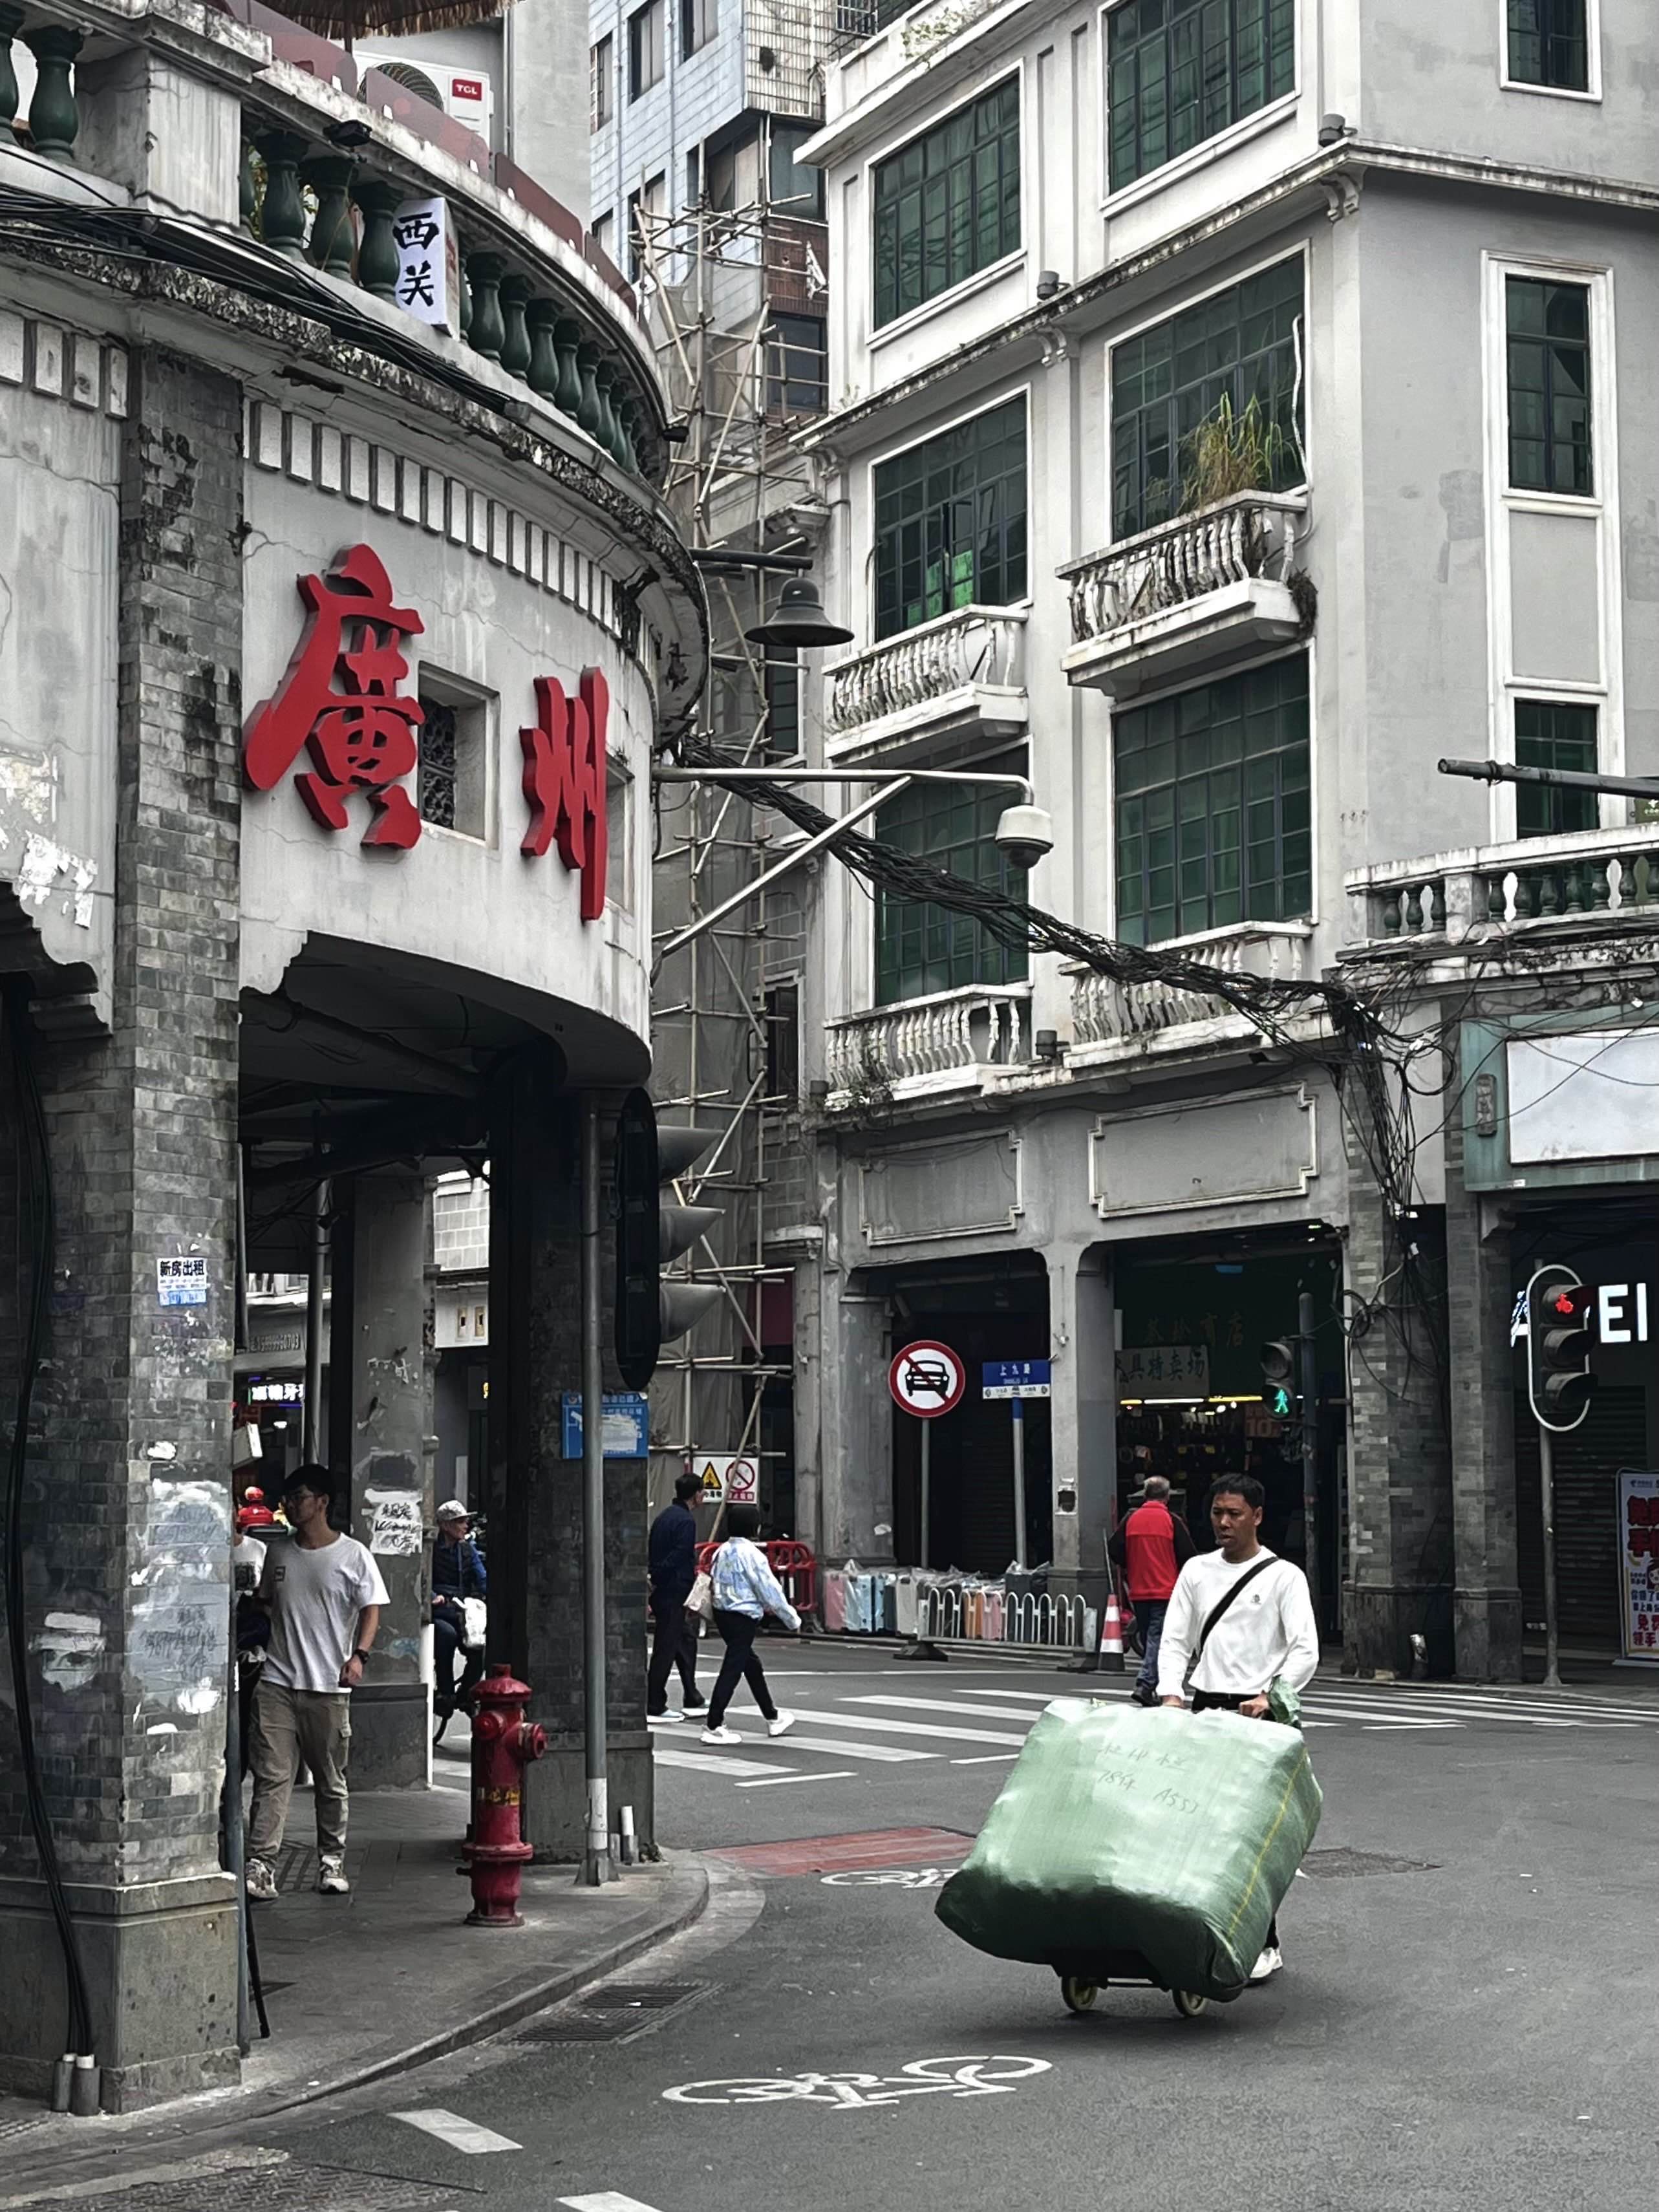
\includegraphics[scale=0.15]{GZXG}\\
\hfill\break
I will end the quarter with one of my favorite pictures taken in my hometown Guangzhou, China.\\ 
\end{center}

\hfill\break
\hfill\break
\noindent Thanks for reading this! Good luck on study, good luck on your exams, and good luck on your career! I hope you enjoy physics, and hope you have learned something from my worksheets :)\\

\end{document}
